%%% Skytools
%%%
%%% SF PUG, July 18 2013
%%%
%%% http://www.meetup.com/postgresql-1/events/125466752/

\documentclass{beamer}

\usepackage[utf8]{inputenc}

\usepackage{minted}
%% \usemintedstyle{emacs}

\usepackage{beamerthemesplit}
\usetheme{Boadilla}
\setbeamertemplate{itemize items}{\checkmark}
\beamertemplatetransparentcovered

\usepackage{multicol}

\title{Skytools3}
\subtitle{PostgreSQL trigger-based replication}
\author{Dimitri Fontaine \texttt{dimitri@2ndQuadrant.fr}}
\date{July, 18 2013}
\logo{
\includegraphics[height=0.4cm]{2ndQuadrant-cross.png}}

\begin{document}

\frame{\titlepage}

\begin{frame}[fragile]
  \frametitle{Dimitri Fontaine}

  \begin{center}
    \textbf{2ndQuadrant France}
    \linebreak
    PostgreSQL Major Contributor
  \end{center}
  \vfill

\begin{columns}[c]
\column{.75\textwidth} 

  \begin{itemize}
   \item<1-> \texttt{pgloader}, \texttt{prefix}, \texttt{skytools}, …
   \item<1-> \texttt{apt.postgresql.org}
   \item<2-> \texttt{\textbf{CREATE EXTENSION}}
   \item<2-> \texttt{\textbf{CREATE EVENT TRIGGER}}
   \item<3-> MySQL migration tool, new \texttt{pgloader} version
  \end{itemize}  

\column{.25\textwidth}
\begin{center}
  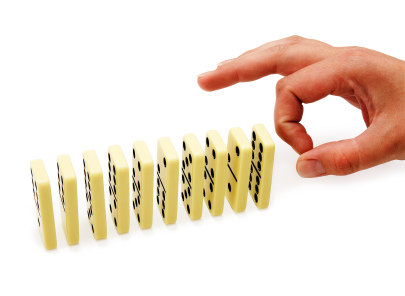
\includegraphics[height=7em]{event-trigger.jpg}
  %% 
\includegraphics[height=5em]{dim-sketch.png}
\end{center}
\end{columns}
\end{frame}

\begin{frame}[fragile]
  \frametitle{Skytools}

  \begin{center}
    \textbf{Skype Tools for Replication}
  \end{center}
  \vfill

\begin{columns}[c]
\column{.45\textwidth} 

  \begin{itemize}
   \item \texttt{PGQ}
   \item \textit{londiste}
   \item \texttt{walmgr}
  \end{itemize}  

\column{.65\textwidth}
\begin{center}
  
\includegraphics[height=1.7in]{skytools3.png}
\end{center}
\end{columns}
\end{frame}

\section{Architecture and concepts}
\subsection{PGQ}

\begin{frame}[fragile]
  \frametitle{Skytools Architecture}

  \begin{center}
    \textbf{PGQ} is organized into 3 components
    \vfill

    Producer, Consumer, Ticker
  \end{center}
\end{frame}

\begin{frame}[fragile]
  \frametitle{PGQ3}

  \center{Some things did change in PGQ \textit{version 3}}
  \vfill

\begin{columns}[c]
\column{.75\textwidth} 

  \begin{itemize}
    \item The ticker is now \texttt{pgqd}
    \item The network topology is now known \texttt{pgq\_nodes}
    \item And we have \textit{Cooperative Consumers} \texttt{pgq\_coop}
  \end{itemize}
\column{.25\textwidth}
\begin{center}
  
\includegraphics[height=5em]{coop-workers.jpeg}
\end{center}
\end{columns}
\end{frame}

\subsection{Londiste}

\begin{frame}[fragile]
  \frametitle{Londiste3 concepts}

  Londiste relies on PGQ nodes
  \vfill

\begin{columns}[c]
\column{.45\textwidth} 

  \begin{itemize}
    \item Root
    \item Branch
    \item Leaf
    \item Leaf --merge='qname'
  \end{itemize}

\column{.65\textwidth}
\begin{center}
  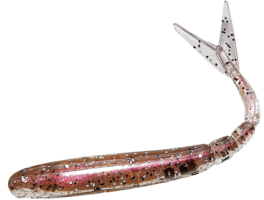
\includegraphics[height=1.7in]{drop-queue.png}
\end{center}
\end{columns}
\end{frame}

\section{Production}
\subsection{Outils}

\begin{frame}[fragile]
  \frametitle{Operating londiste}

  \center{Basic commands}
  \vfill

\begin{columns}[c]
\column{.45\textwidth} 

  \begin{itemize}
    \item \texttt{status}
    \item \texttt{members}
    \item \texttt{change-provider}
    \item \texttt{takeover} \textit{--all} \textit{--dead}
  \end{itemize}

\column{.65\textwidth}
\begin{center}
  
\includegraphics[height=1.4in]{TerminalIcon.png}
\end{center}
\end{columns}
\end{frame}

\subsection{add-table}

\begin{frame}[fragile]
  \frametitle{Londiste Add Table}

  \begin{center}
    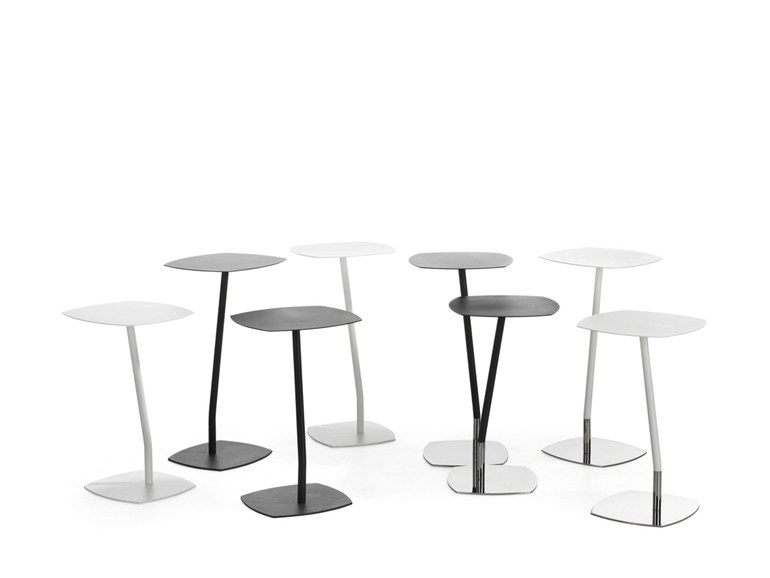
\includegraphics[height=21em] {add-table.jpg}
  \end{center}
\end{frame}

\frame{
  \frametitle{\texttt{londiste add-table}}

  Plenty new options in \texttt{add-table}

  \begin{multicols}{2}
    \begin{itemize}
      \item \texttt{--wait-sync}
      \item \texttt{--dest-table}
      \item \texttt{--skip-truncate}
      \item \texttt{--create, --create-full}
      \item \texttt{--trigger-flags}
      \item \texttt{--trigger-arg}
      \item \texttt{--no-triggers}
      \item \texttt{--copy-node, --copy-condition}
      \item \texttt{--merge-all, --no-merge}
      \item \texttt{--max-parallel-copy}
    \end{itemize}
  \end{multicols}
}

\subsection{execute}

\begin{frame}[fragile]
  \frametitle{DDL}

  \begin{center}
    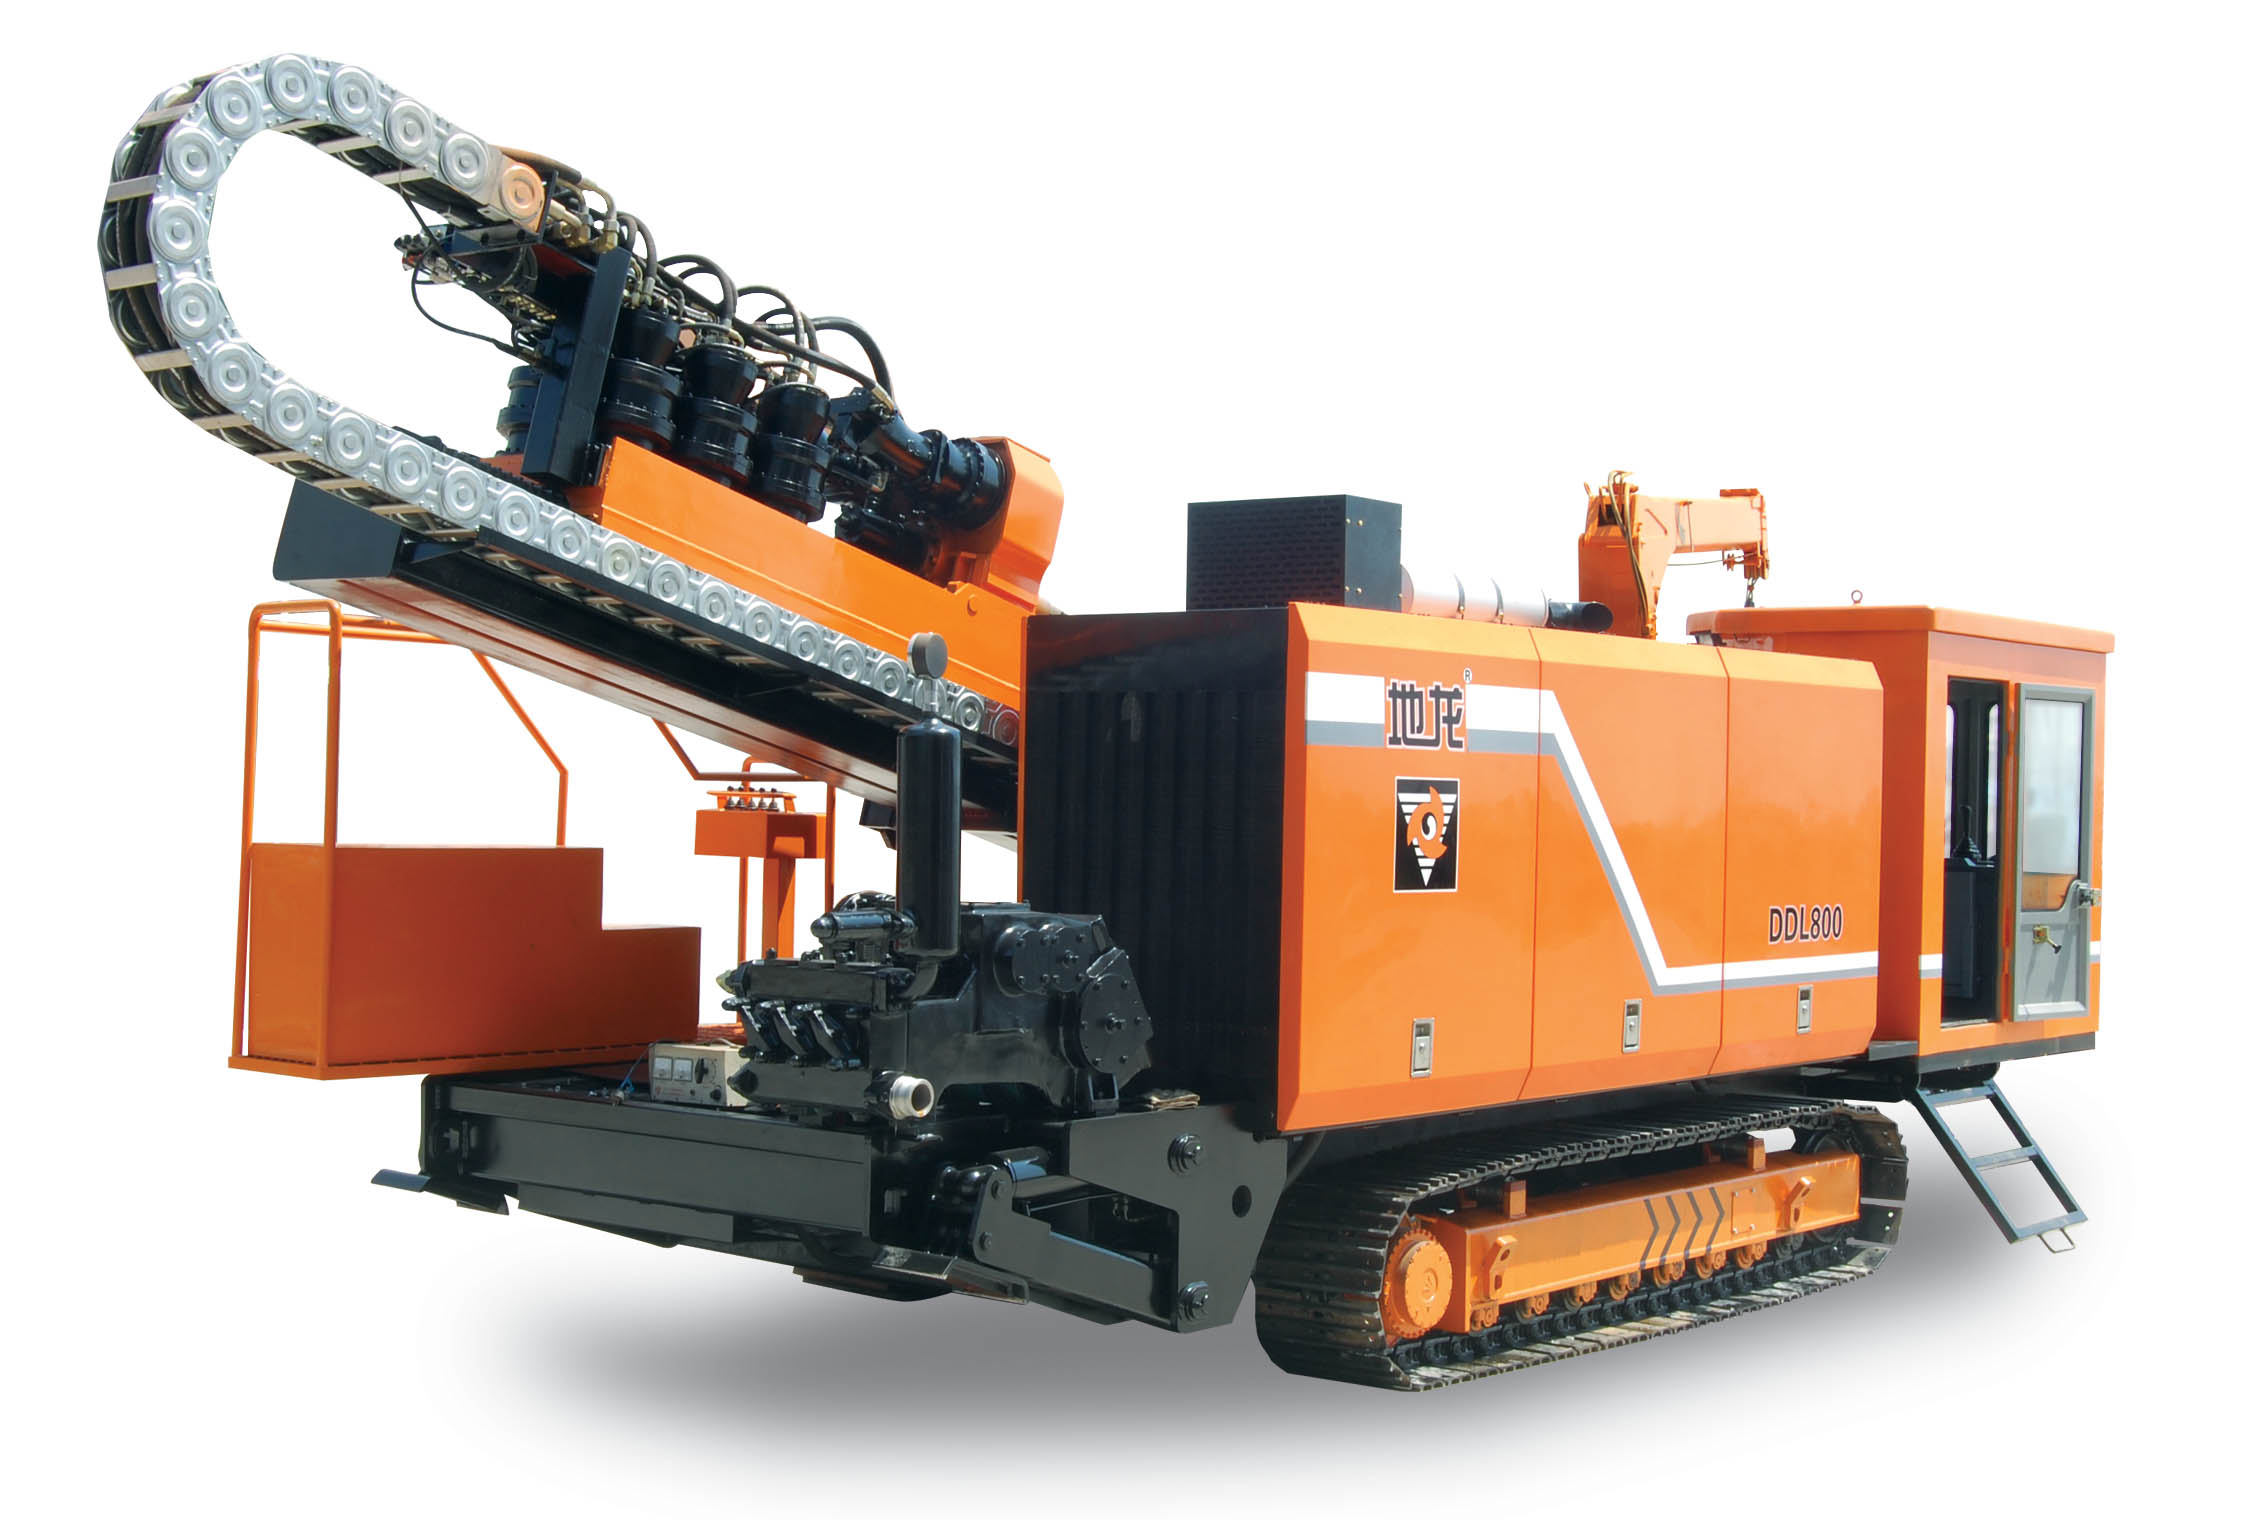
\includegraphics[height=21em]
                    {Horizontal-Directional-Drilling-Rig-DDL-800-.jpg}
  \end{center}
\end{frame}

\begin{frame}[fragile]
  \frametitle{DDL Handling}

\begin{columns}[c]
\column{.8\textwidth} 

  \begin{itemize}
    \item \texttt{londiste conf.ini execute}
    \item \texttt{EXECUTE} queue events
    \item \textit{System Table} \texttt{londiste.applied\_execute}
    \item SQL meta-data attributes
  \end{itemize}

\column{.2\textwidth}
\begin{center}
  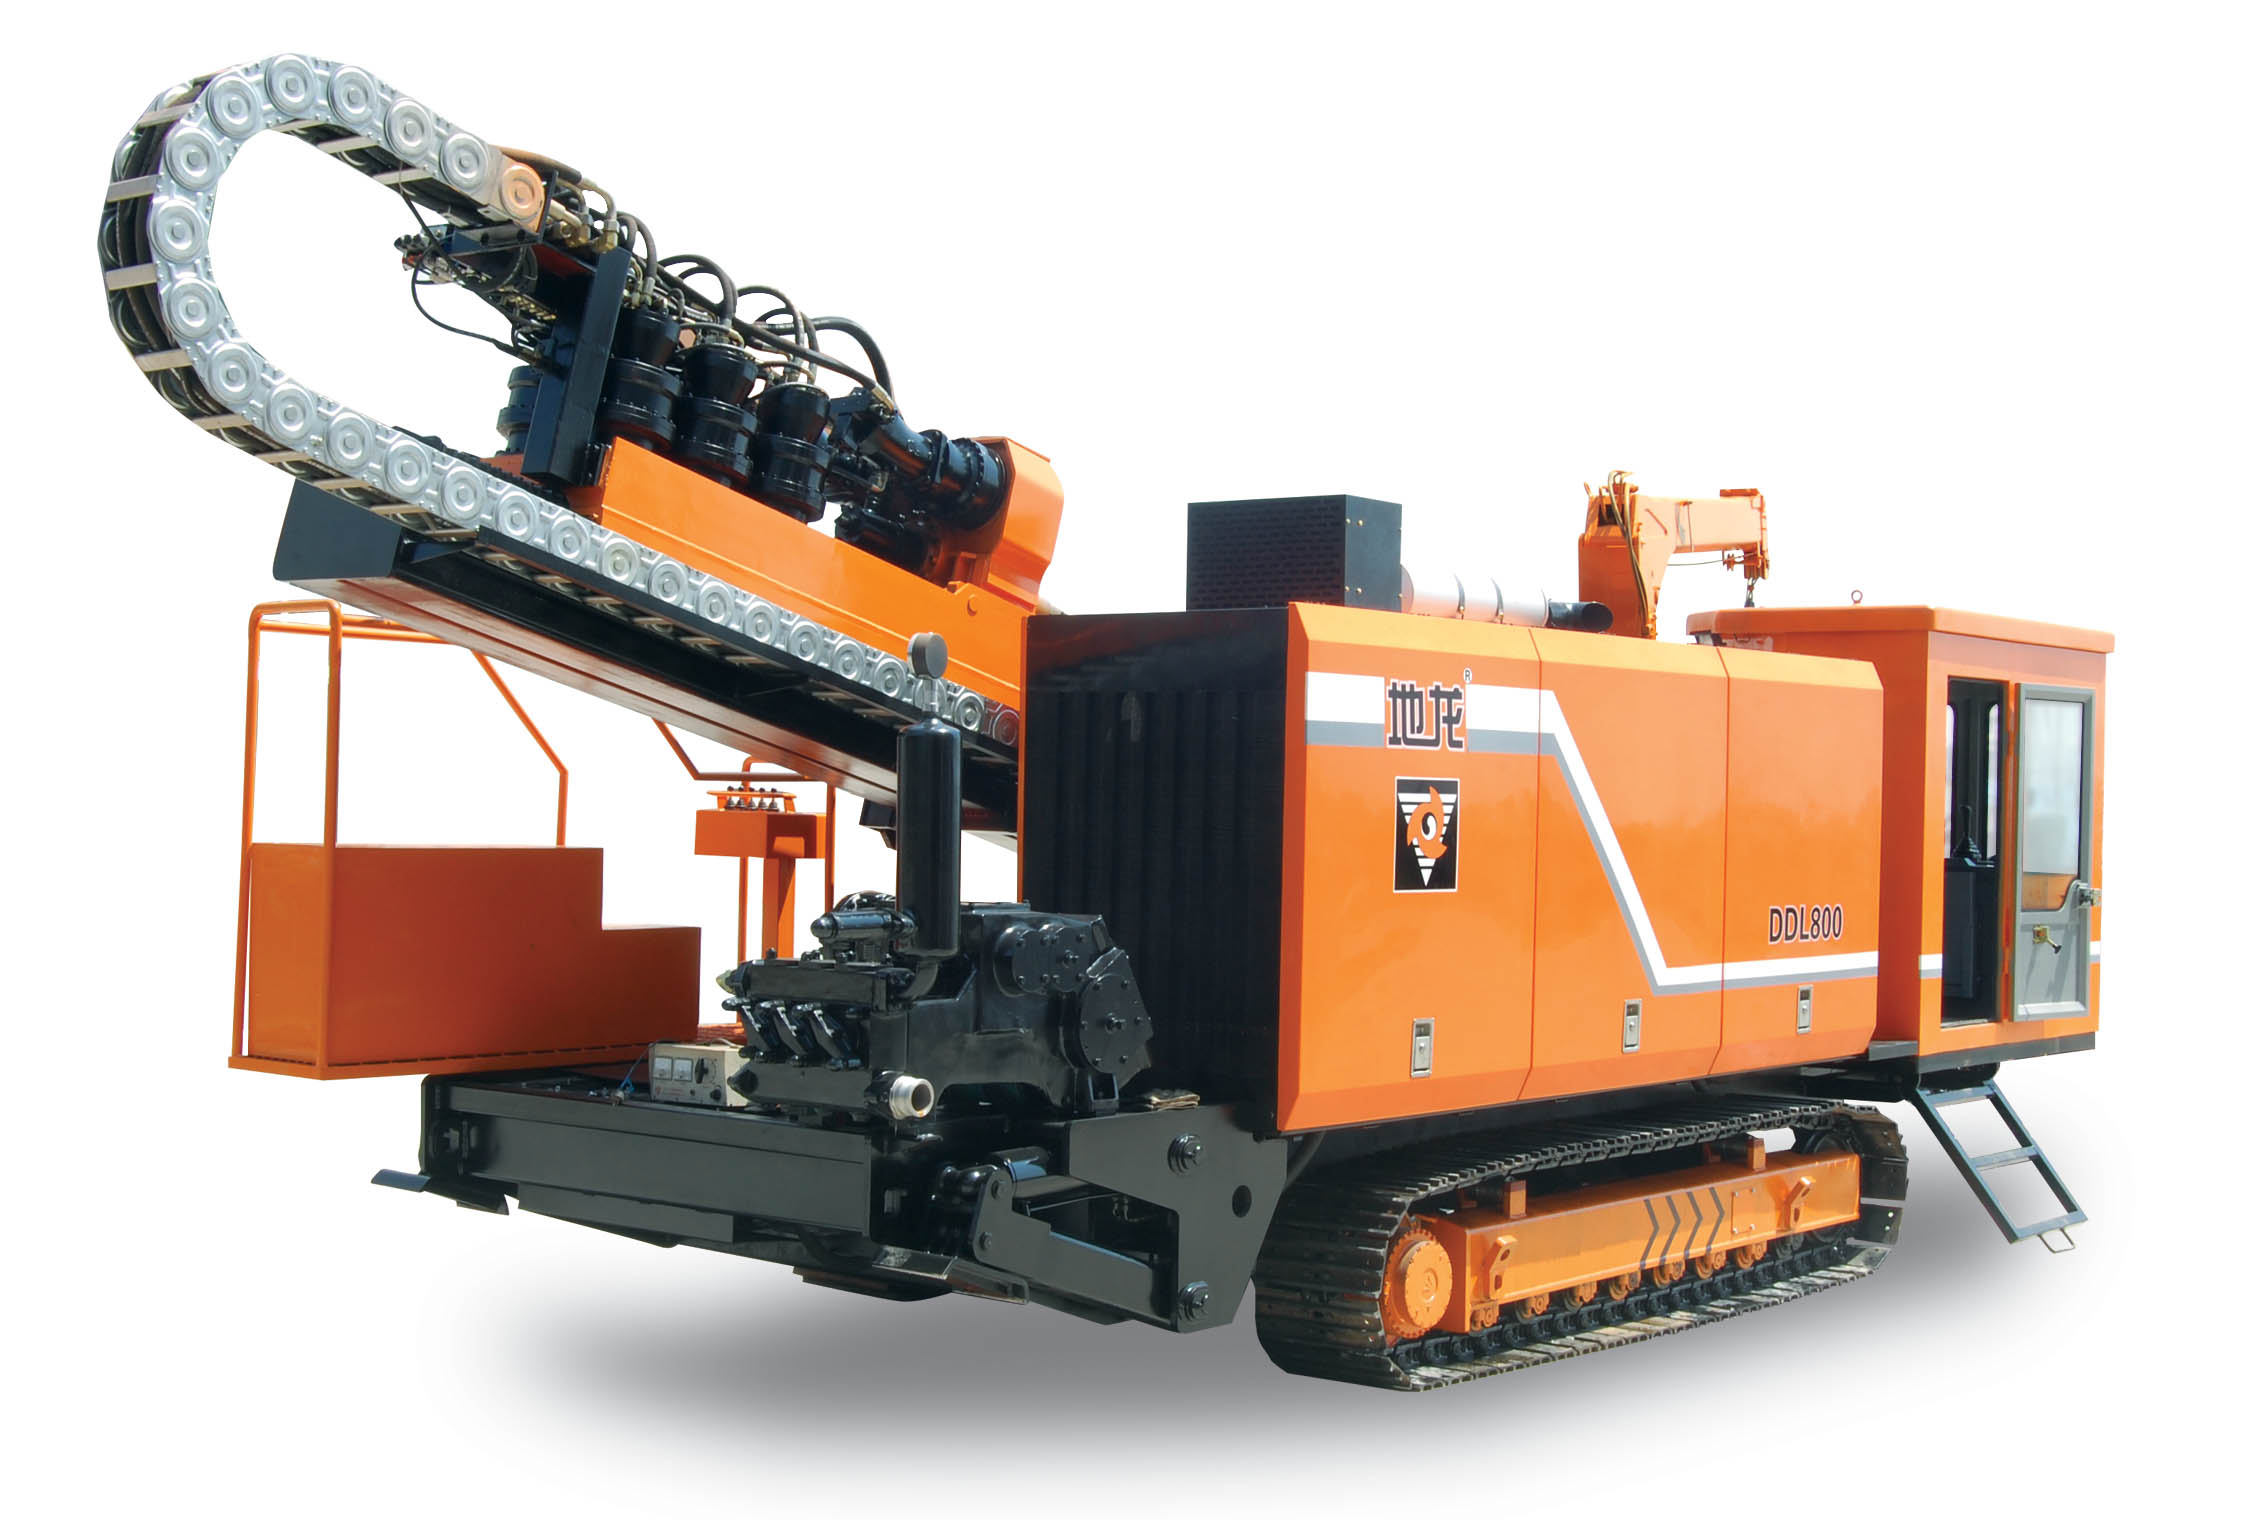
\includegraphics[height=4em]{Horizontal-Directional-Drilling-Rig-DDL-800-.jpg}
\end{center}
\end{columns}
\end{frame}

\begin{frame}[fragile]{execute Meta-Data attributes}
\begin{minted}{postgresql}
  --*--
  --*-- Local-Table: mytable, othertable,
  --*--              thirdtable
  --*-- Local-Sequence: thisseq
  --*--
\end{minted}

\begin{itemize}
\item \textit{Local-Table}
  Table must be added to local node with \texttt{add-table}.
\item \textit{Need-Table}
    Physical table must exist in database.  It does not matter if it is
    replicated or not.
\end{itemize}
\end{frame}

\begin{frame}[fragile]{DDL and table renaming}
  
\begin{minted}{postgresql}
  --*-- Local-Table: mytable
  ALTER TABLE @mytable@ ...;
\end{minted}

\end{frame}

\section{Londiste Handlers}
\subsection{Concepts et commandes}

\begin{frame}[fragile]
  \frametitle{Londiste Handlers}

  \center{It's possible to register handlers to deal with specific needs}
  \vfill

\begin{columns}[c]
\column{.75\textwidth} 

  \begin{itemize}
    \item \texttt{add --handler [ --handler-arg ... ] }
    \item \texttt{show-handlers}
    \item pl/proxy sharding, re-sharding
  \end{itemize}

\column{.25\textwidth}
\begin{center}
  
\includegraphics[height=1.5in]{plugin.jpg}
\end{center}
\end{columns}
\end{frame}

\subsection{Partitionnement}

\begin{frame}[fragile]
  \frametitle{Sharding pluging}

  \begin{center}
    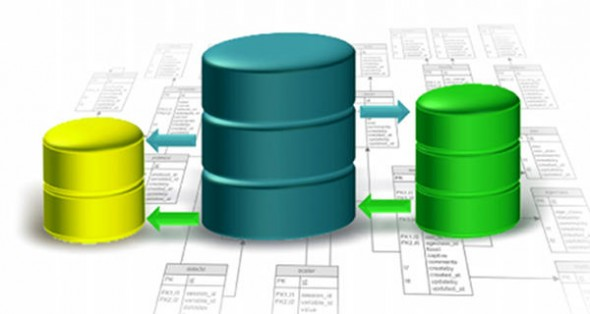
\includegraphics[height=16em] {partitioning-in-podtgre-590x314.jpg}
  \end{center}
\end{frame}

\begin{frame}[fragile]
  \frametitle{Handler: shard}

  \begin{itemize}
    \item Event filtering by hash, for partitioned databases.
    \item \texttt{key=COLUMN} column name to use for hashing
    \item \texttt{hashfunc=FUNCNAME} function to use for hashing
    \item (default: \texttt{partconf.get\_hash\_raw})
    \item \texttt{ev\_extra3='hash='||partconf.get\_hash\_raw(key\_column)}
  \end{itemize}
\end{frame}

\begin{frame}[fragile]{Preparing for part: hashlib}
\begin{minted}{console}
> ... add-table pgbench_accounts \
>  --handler=part --handler-arg=key=aid

psql rootdb < /usr/share/postgresql/8.4/contrib/hashlib.sql 
psql sharddb_0 < /usr/share/postgresql/8.4/contrib/hashlib.sql 
psql sharddb_1 < /usr/share/postgresql/8.4/contrib/hashlib.sql 

> psql rootdb -c 'create extension hashlib;'
> psql sharddb_0 -c 'create extension hashlib;'
> psql sharddb_1 -c 'create extension hashlib;'
\end{minted}
\end{frame}

\begin{frame}[fragile]{Preparing for part: setup}
\begin{minted}{postgresql}
CREATE SCHEMA partconf;

CREATE TABLE partconf.conf (
    part_nr integer,
    max_part integer,
    db_code bigint,
    is_primary boolean,
    max_slot integer,
    cluster_name text
);
\end{minted}
\end{frame}

\begin{frame}[fragile]{Preparing for part: get\_hash\_raw}
\begin{minted}{postgresql}
CREATE FUNCTION partconf.get_hash_raw
 ( i_input integer)
 RETURNS integer
 LANGUAGE sql
AS $$
-- used to wrap hashtext so that we can replace it in 8.4
-- with older implementation to keep compatibility
select hash_string(\$1::text, 'lookup2');
$$;
\end{minted}
\end{frame}

\begin{frame}[fragile]{Preparing for part: local\_part}
\begin{minted}{console}
> psql rootdb < partconf.sql
> psql sharddb_0 < partconf.sql
> psql sharddb_1 < partconf.sql

> psql sharddb_0
=> insert into partconf.conf(part_nr, max_part)
        values (0,1);

> psql sharddb_1
=> insert into partconf.conf(part_nr, max_part)
        values (1,1);
\end{minted}
\end{frame}

\begin{frame}[fragile]{Preparing for part: add-table}
\begin{minted}{console}
> londiste3 st3partsplit/st3_rootdb.ini
  add-table pgbench_accounts
  --handler=part --handler-arg=key=aid

> londiste3 st3partsplit/st3_sharddb_0.ini
  add-table pgbench_accounts --create
  --handler=part --handler-arg=key=aid

> londiste3 st3partsplit/st3_sharddb_1.ini
  add-table pgbench_accounts --create
  --handler=part --handler-arg=key=aid
\end{minted}
\end{frame}

\subsection{Autres Handlers}

\frame{
  \frametitle{Other Handlers}

  \begin{multicols}{2}
    \begin{itemize}
      \item \texttt{applyfn}
      \item \texttt{bulk}
      \item \texttt{dispatch}
      \item \texttt{multimaster}
      \item \texttt{part}
      \item \texttt{qtable}
      \item \texttt{vtable}
    \end{itemize}
  \end{multicols}
}

\subsection{bulk loading}

\begin{frame}[fragile]
  \frametitle{Handler: bulk}

  \center{bulk loading with 3 options}
  \vfill
  
\begin{columns}[c]
\column{.75\textwidth} 

  \begin{itemize}
    \item correct: COPY, COPY temp + UPDATE, COPY temp + DELETE
    \item delete: correct + update devient DELETE + COPY
    \item merged: merge insert rows with update rows
  \end{itemize}

\column{.25\textwidth}
\begin{center}
  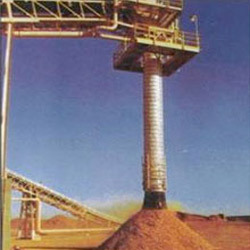
\includegraphics[height=6em]{2bulk-loading-spout-250x250.jpg}
\end{center}
\end{columns}
\end{frame}

\begin{frame}[fragile]
  \frametitle{Handler: dispatch}

  \center{\texttt{bulk\_monthly\_batch}}
  \vfill

\begin{columns}[c]
\column{.5\textwidth} 

  \begin{itemize}
    \item bulk
    \item hourly daily monthly yearly
    \item event batch field time
  \end{itemize}

\column{.5\textwidth}
\begin{center}
  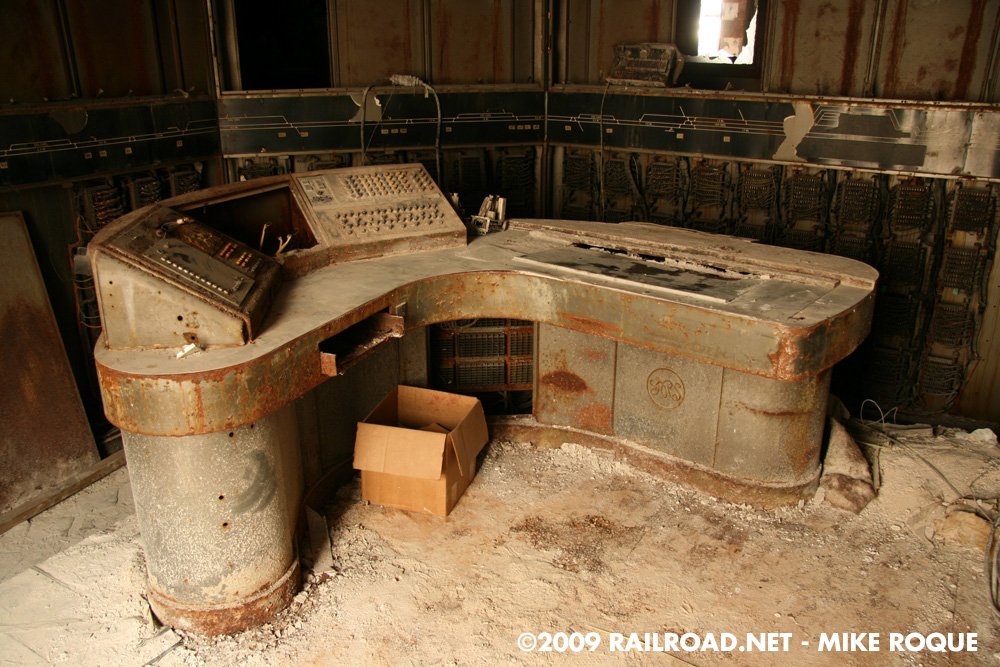
\includegraphics[height=9em]{BCT_DispatcherDesk_Large.jpg}
\end{center}
\end{columns}
\end{frame}

\frame{
  \frametitle{Handler: dispatch}

  \begin{multicols}{2}
  \begin{itemize}
    \item \texttt{table\_mode} part, direct, ignore
    \item \texttt{part\_mode} batch\_time, event, time, date\_field, current\_time
    \item \texttt{part\_field} date\_field
    \item \texttt{period} hour, day, month, year
    \item \texttt{row\_mode} plain, keep\_latest, keep\_all
    \item \texttt{event\_types} I,U,D
    \item \texttt{load\_mode} direct, bulk
    \item \texttt{method} correct, delete, merged, insert
    \item \texttt{fields} field name mapping, no COPY support
    \item \texttt{skip\_fields}
    \item \texttt{table}
    \item \texttt{pre\_part}, \texttt{post\_part}
    \item \texttt{encoding}
    \item \texttt{analyze}
  \end{itemize}
  \end{multicols}
}

\section{Londiste Extras}

\begin{frame}[fragile]
  \frametitle{Extras}

\begin{columns}[c]
\column{.75\textwidth} 

  \begin{multicols}{2}
    \begin{itemize}
      \item \texttt{check}
      \item \texttt{fkeys}
      \item \texttt{compare}
      \item \texttt{repair}
      \item \texttt{wait-sync}
      \item \texttt{wait-provider}
      \item \texttt{wait-root}
    \end{itemize}
   \end{multicols}

\column{.25\textwidth}
\begin{center}
  
\includegraphics[height=6em]{extra.jpg}
\end{center}
\end{columns}
\end{frame}

\section{Conclusion}

\frame{
  \frametitle{Questions?}

\begin{center}
  Now is the time to ask!
  \vfill

  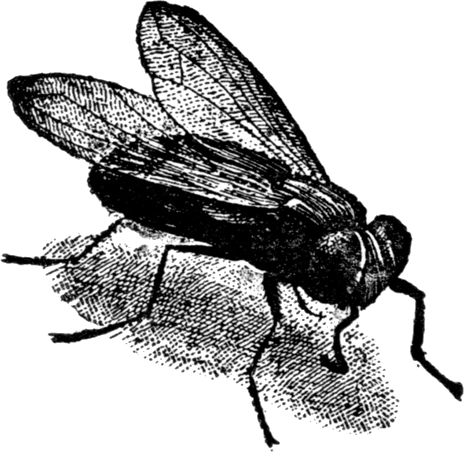
\includegraphics[height=9em]{fly.png}
\end{center}
}

\end{document}
